\documentclass[tikz,border=6pt]{standalone}
\usepackage{amsmath,amssymb,mathtools,physics,bm,nicefrac,wasysym}
\usepackage{xcolor}

\definecolor{colone}{RGB}{180,60,60}
\definecolor{coltwo}{RGB}{60,110,180}
\definecolor{colthree}{RGB}{60,140,80}

\definecolor{accent}{HTML}{A13D2C}
\definecolor{accent2}{HTML}{2B5F6B}
\definecolor{muted}{HTML}{5A564F}
\definecolor{panel}{HTML}{F8F6F0}
\definecolor{linecol}{HTML}{D8D2C4}
\definecolor{ink}{HTML}{1E1C1A}
\definecolor{astroblue}{HTML}{1B4F72}
\definecolor{astrodark}{HTML}{17202A}
\definecolor{sunyellow}{HTML}{E8A33D}

\usetikzlibrary{calc,arrows.meta,positioning,decorations.pathreplacing,decorations.markings,angles,quotes,shapes.geometric}
\usepackage{tikz-3dplot}

\newcommand{\vecr}{\vec r}
\newcommand{\vecL}{\vec L}
\newcommand{\vecA}{\vec A}
\newcommand{\vecf}{\vec f}
\newcommand{\vecF}{\vec F}
\newcommand{\vecp}{\vec p}
\newcommand{\avg}[1]{\left\langle #1\right\rangle}
\newcommand{\vecx}{\vec x}
\newcommand{\hatn}{\hat n}
\newcommand{\rhat}{\hat r}
\newcommand{\phihat}{\hat\phi}
\newcommand{\thetahat}{\hat\theta}
\newcommand{\note}[1]{\textcolor{blue!60!black}{\textit{[#1]}}}

\newcommand{\LST}{\mathrm{LST}}
\newcommand{\GST}{\mathrm{GST}}
\newcommand{\GMST}{\mathrm{GMST}}
\newcommand{\GAST}{\mathrm{GAST}}
\newcommand{\LMST}{\mathrm{LMST}}
\newcommand{\LAST}{\mathrm{LAST}}
\newcommand{\UT}{\mathrm{UT}}
\newcommand{\UTC}{\mathrm{UTC}}
\newcommand{\TAI}{\mathrm{TAI}}
\newcommand{\TT}{\mathrm{TT}}
\newcommand{\TDB}{\mathrm{TDB}}
\newcommand{\JD}{\mathrm{JD}}
\newcommand{\MJD}{\mathrm{MJD}}
\newcommand{\EoT}{\mathrm{EoT}}
\newcommand{\SNR}{\mathrm{SNR}}
\newcommand{\RON}{\mathrm{RON}}



\begin{document}
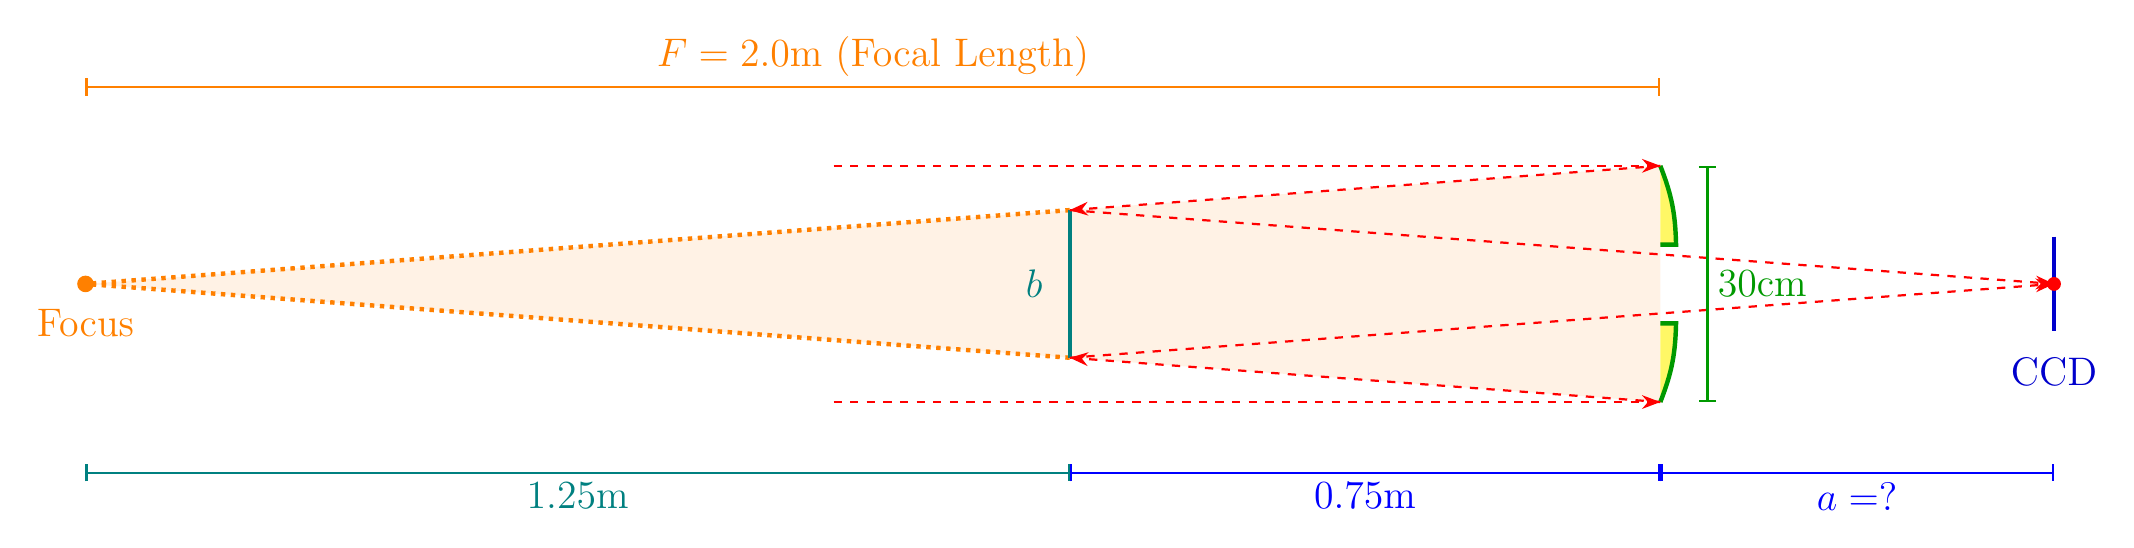
\begin{tikzpicture}[scale=1.0, >=Stealth]
    \def\D{3.0}     % Primary diameter (30 cm scaled)
    \def\d{7.5}     % Mirror distance (0.75 m scaled)
    \def\b{1.875}   % Secondary diameter (18.75 cm scaled)
    \def\a{5.0}     % CCD distance (0.5 m scaled)
    \def\F{-12.5}   % Primary focus (2.0 m scaled -> 20 units left of primary at 7.5)
    
    % Background shading for the similar triangle
    \fill[orange!10] (\d, 1.5) -- (\F, 0) -- (\d, -1.5) -- cycle;
    
    % Virtual rays continuing to the Primary Focus (completes the similar triangle)
    \draw[dotted, orange, ultra thick] (0, \b/2) -- (\F, 0);
    \draw[dotted, orange, ultra thick] (0, -\b/2) -- (\F, 0);
    \fill[orange] (\F, 0) circle (3pt) node[below=2mm] {\Large Focus};
    
    % Mark overall Focal Length (F = 2.0m) at the top
    \draw[|-|, thick, orange] (\F, 2.5) -- (\d, 2.5) node[midway, above] {\Large $F = 2.0\text{m}$ (Focal Length)};

    % Incoming Rays from infinity (aligned with the edges of the primary mirror)
    \draw[dashed, red, thick, ->] (-3, 1.5) -- (\d, 1.5);
    \draw[dashed, red, thick, ->] (-3, -1.5) -- (\d, -1.5);
    
    % Primary Mirror
    \fill[yellow!60] (\d, 1.5) to[bend left=10] (\d+0.2, 0.5) -- (\d, 0.5) -- cycle;
    \fill[yellow!60] (\d, -1.5) to[bend right=10] (\d+0.2, -0.5) -- (\d, -0.5) -- cycle;
    \draw[ultra thick, green!60!black] (\d, 1.5) to[bend left=10] (\d+0.2, 0.5) -- (\d, 0.5);
    \draw[ultra thick, green!60!black] (\d, -1.5) to[bend right=10] (\d+0.2, -0.5) -- (\d, -0.5);
    
    % Secondary Mirror
    \draw[ultra thick, teal] (0, \b/2) -- (0, -\b/2) node[midway, left=2mm, text=teal] {\Large $b$};
    
    % Reflected converging rays from primary to secondary
    \draw[dashed, red, thick, ->] (\d, 1.5) -- (0, \b/2);
    \draw[dashed, red, thick, ->] (\d, -1.5) -- (0, -\b/2);
    
    % Reflected rays from secondary to CCD
    \draw[dashed, red, thick, ->] (0, \b/2) -- (\d+\a, 0);
    \draw[dashed, red, thick, ->] (0, -\b/2) -- (\d+\a, 0);
    
    % CCD at focal plane
    \draw[ultra thick, blue!80!black] (\d+\a, 0.6) -- (\d+\a, -0.6) node[below=2mm] {\Large CCD};
    \fill[red] (\d+\a, 0) circle (2.5pt);
    
    % Continuous bottom dimension lines showing the geometry
    \draw[|-|, thick, teal] (\F, -2.4) -- (0, -2.4) node[midway, below] {\Large $1.25\text{m}$};
    \draw[|-|, thick, blue] (0, -2.4) -- (\d, -2.4) node[midway, below] {\Large $0.75\text{m}$};
    \draw[|-|, thick, blue] (\d, -2.4) -- (\d+\a, -2.4) node[midway, below] {\Large $a=?$};
    
    % Primary Mirror Aperture Dimension
    \draw[|-|, thick, green!60!black] (\d+0.6, -1.5) -- (\d+0.6, 1.5) node[midway, right] {\Large $30\text{cm}$};
\end{tikzpicture}
\end{document}
